
% BOILERPLATE - Allows for individual chapters to be compiled.
%
% Usage:
%    % BOILERPLATE - Allows for individual chapters to be compiled.
%
% Usage:
%    % BOILERPLATE - Allows for individual chapters to be compiled.
%
% Usage:
%    \input{../settings/boilerplate} % place at start and end of chapter
% 

\def\precommands{%
    \input{../settings/phdsetup}
    \def\preinserted{}
    \begin{document}
}

\def\postcommands{%
    \singlespacing
    \phantomsection
%    \bibliographystyle{../bibliography/expanded}
   \bibliographystyle{elsarticle-harv}
   \bibliography{../bibliography/references}
    \enddocument
}

\def\autoinsert{%
    \ifx\preinserted\undefined
        \expandafter\precommands
    \else
        \expandafter\postcommands
    \fi
}

\ifx\master\undefined\expandafter\autoinsert\fi

 % place at start and end of chapter
% 

\def\precommands{%
    % [ USER VARIABLES ]

\def\PHDTITLE {Regime shifts in ecology and evolution}
\def\PHDAUTHOR{Carl Boettiger}
\def\PHDSCHOOL{University of California, Davis}

\def\PHDMONTH {September}
\def\PHDYEAR  {2012}
\def\PHDDEPT {Center for Population Biology}

\def\BSSCHOOL {Princeton}
\def\BSYEAR   {2007}

\def\PHDCOMMITTEEA{Alan Hastings}
\def\PHDCOMMITTEEB{Peter Wainwright}
\def\PHDCOMMITTEEC{Brian Moore}

% [ GLOBAL SETUP ]

\documentclass[letterpaper,oneside,11pt]{report}


% [ CARL BOETTIGER`S CUSTOM COMMANDS, LIBRARIES, ETC ]

\usepackage{subfigure}
\usepackage[sort&compress]{natbib}
\usepackage{color}
\usepackage{fancyvrb}
\usepackage{ctable}


\usepackage{silence}
\WarningFilter{amsmath}{Underfull}     

%\newcommand{\argmax}{\operatorname{argmax}}
\newcommand{\ud}{\mathrm{d}}


\usepackage{calc}
\usepackage{breakcites}
\usepackage[newcommands]{ragged2e}
\usepackage{appendix}
\usepackage{comment}
\usepackage{xifthen}

\usepackage{graphicx}
\usepackage{epstopdf}


\renewenvironment{abstract}{\chapter*{Abstract}}{}
\renewcommand{\bibname}{Bibliography}
\renewcommand{\contentsname}{Table of Contents}

\makeatletter
\renewcommand{\@biblabel}[1]{\textsc{#1}}
\makeatother

% [ FONT SETTINGS ]

\usepackage[T1]{fontenc}
\usepackage{libertine}

\usepackage[tbtags, intlimits, namelimits]{amsmath}
\usepackage{amsthm}
\usepackage{amssymb}
\usepackage{amsfonts}



% [ PAGE LAYOUT ]

\usepackage{geometry}
\geometry{lmargin = 1.5in}
\geometry{rmargin = 1.0in}
\geometry{tmargin = 1.0in}
\geometry{bmargin = 1.0in}

% [ PDF SETTINGS ]

\usepackage[final]{hyperref}
\hypersetup{
    breaklinks  = {true},
    colorlinks  = {true},
    linktocpage = {false},
    linkcolor   = {blue},
    citecolor   = {black},
    urlcolor    = {black},
    plainpages  = {false},
    pageanchor  = {true},
    pdfauthor   = {\PHDAUTHOR},
    pdftitle    = {\PHDTITLE},
    pdfsubject  = {Dissertation, \PHDSCHOOL},
    pdfcreator  = {},
    pdfkeywords = {},
    pdfproducer = {}
}
\urlstyle{same}

% [ LETTER SPACING ]

\usepackage[final]{microtype}
\microtypesetup{protrusion=compatibility}
\microtypesetup{expansion=false}

\newcommand{\upper}[1]{\MakeUppercase{#1}}
\let\lsscshape\scshape

\ifcase\pdfoutput\else\microtypesetup{letterspace=15}
\renewcommand{\scshape}{\lsscshape\lsstyle}
\renewcommand{\upper}[1]{\textls[50]{\MakeUppercase{#1}}}\fi

% [ LINE SPACING ]

\usepackage[doublespacing]{setspace}
\renewcommand{\displayskipstretch}{0.75}

\setlength{\parskip   }{0em}
\setlength{\parindent }{2em}

% [ TABLE FORMATTING ]

\usepackage{booktabs}
\usepackage{multirow}
\usepackage{dcolumn}
\setlength{\heavyrulewidth}{1.5\arrayrulewidth}
\setlength{\lightrulewidth}{1.0\arrayrulewidth}
\setlength{\doublerulesep }{2.0\arrayrulewidth}

% [ SECTION FORMATTING ]

\usepackage[largestsep,nobottomtitles*]{titlesec}
\renewcommand{\bottomtitlespace}{0.75in}

\titleformat{\chapter}[display]%
    {\bfseries\huge\singlespacing}%
    {\filleft\textsc{\LARGE \chaptertitlename\ \thechapter}}%
    {-0.2ex}{\titlerule[3pt]\vspace{0.2ex}}[]

\titleformat{\section}{\LARGE}{\thesection\hspace{0.5em}}{0ex}{}
\titleformat{\subsection}{\Large}{\thesubsection\hspace{0.5em}}{0ex}{}
\titleformat{\subsubsection}{\large}{\thesubsubsection\hspace{0.5em}}{0ex}{}

\titlespacing*{\chapter}{0em}{6ex}{4ex plus 2ex minus 0ex}
\titlespacing*{\section}{0em}{2ex plus 3ex minus 1ex}{0.5ex plus 0.5ex minus 0.5ex}
\titlespacing*{\subsection}{0ex}{2ex plus 3ex minus 1ex}{0ex}
\titlespacing*{\subsubsection}{0ex}{2ex plus 0ex minus 1ex}{0ex}

% [ HEADER SETTINGS ]

\usepackage{fancyhdr}

\setlength{\headheight}{\normalbaselineskip}
\setlength{\footskip  }{0.5in}
\setlength{\headsep   }{0.5in-\headheight}

\fancyheadoffset[R]{0.5in}
\renewcommand{\headrulewidth}{0pt}
\renewcommand{\footrulewidth}{0pt}

\newcommand{\pagebox}{\parbox[r][\headheight][t]{0.5in}{\hspace\fill\thepage}}

\newcommand{\prelimheaders}{\ifx\prelim\undefined\renewcommand{\thepage}{\textit{\roman{page}}}\fancypagestyle{plain}{\fancyhf{}\fancyfoot[L]{\makebox[\textwidth-0.5in]{\thepage}}}\pagestyle{plain}\def\prelim{}\fi}

\newcommand{\normalheaders}{\renewcommand{\thepage}{\arabic{page}}\fancypagestyle{plain}{\fancyhf{}\fancyhead[R]{\pagebox}}\pagestyle{plain}}

\normalheaders{}

% [ CUSTOM COMMANDS ]

\newcommand{\signaturebox}[1]{\multicolumn{1}{p{4in}}{\vspace{3ex}}\\\midrule #1\\}

% Redefine AMS proof environment to have itshape
% Note: This environment automatically adds \qed at the end. If your proof
% ends in a math environment, the \qed is placed, undesirably, on a new line.
% To prevent that, insert \qedhere inside the math environment.
\makeatletter
\renewenvironment{proof}[1][\proofname]{%
\par\pushQED{\qed}\normalfont%
\topsep6\p@\@plus6\p@\relax\trivlist%
\item[\hskip\labelsep\bfseries#1\@addpunct{.}]\itshape\ignorespaces}{%
\popQED\endtrivlist\@endpefalse}%
\makeatother

% TUGboat, Volume 0 (2001), No. 0
% http://math.arizona.edu/~aprl/publications/mathclap/perlis_mathclap_24Jun2003.pdf
% For comparison, here are the existing overlap macros:
% \def\llap#1{\hbox to 0pt{\hss#1}}
% \def\rlap#1{\hbox to 0pt{#1\hss}}
\def\clap#1{\hbox to 0pt{\hss#1\hss}}
\def\mathllap{\mathpalette\mathllapinternal}
\def\mathrlap{\mathpalette\mathrlapinternal}
\def\mathclap{\mathpalette\mathclapinternal}
\def\mathllapinternal#1#2{%
\llap{$\mathsurround=0pt#1{#2}$}}
\def\mathrlapinternal#1#2{%
\rlap{$\mathsurround=0pt#1{#2}$}}
\def\mathclapinternal#1#2{%
\clap{$\mathsurround=0pt#1{#2}$}}

\newcommand{\alert}[1]{\textbf{\textcolor{red}{#1}}}




% [ Code blocks ]
%\DefineShortVerb[commandchars=\\\{\}]{\|}
\DefineVerbatimEnvironment{Highlighting}{Verbatim}{commandchars=\\\{\}}
% Add ',fontsize=\small' for more characters per line
\newenvironment{Shaded}{}{}
\newcommand{\KeywordTok}[1]{\textcolor[rgb]{0.00,0.44,0.13}{\textbf{{#1}}}}
\newcommand{\DataTypeTok}[1]{\textcolor[rgb]{0.56,0.13,0.00}{{#1}}}
\newcommand{\DecValTok}[1]{\textcolor[rgb]{0.25,0.63,0.44}{{#1}}}
\newcommand{\BaseNTok}[1]{\textcolor[rgb]{0.25,0.63,0.44}{{#1}}}
\newcommand{\FloatTok}[1]{\textcolor[rgb]{0.25,0.63,0.44}{{#1}}}
\newcommand{\CharTok}[1]{\textcolor[rgb]{0.25,0.44,0.63}{{#1}}}
\newcommand{\StringTok}[1]{\textcolor[rgb]{0.25,0.44,0.63}{{#1}}}
\newcommand{\CommentTok}[1]{\textcolor[rgb]{0.38,0.63,0.69}{\textit{{#1}}}}
\newcommand{\OtherTok}[1]{\textcolor[rgb]{0.00,0.44,0.13}{{#1}}}
\newcommand{\AlertTok}[1]{\textcolor[rgb]{1.00,0.00,0.00}{\textbf{{#1}}}}
\newcommand{\FunctionTok}[1]{\textcolor[rgb]{0.02,0.16,0.49}{{#1}}}
\newcommand{\RegionMarkerTok}[1]{{#1}}
\newcommand{\ErrorTok}[1]{\textcolor[rgb]{1.00,0.00,0.00}{\textbf{{#1}}}}
\newcommand{\NormalTok}[1]{{#1}}



    \def\preinserted{}
    \begin{document}
}

\def\postcommands{%
    \singlespacing
    \phantomsection
%    \bibliographystyle{../bibliography/expanded}
   \bibliographystyle{elsarticle-harv}
   \bibliography{../bibliography/references}
    \enddocument
}

\def\autoinsert{%
    \ifx\preinserted\undefined
        \expandafter\precommands
    \else
        \expandafter\postcommands
    \fi
}

\ifx\master\undefined\expandafter\autoinsert\fi

 % place at start and end of chapter
% 

\def\precommands{%
    % [ USER VARIABLES ]

\def\PHDTITLE {Regime shifts in ecology and evolution}
\def\PHDAUTHOR{Carl Boettiger}
\def\PHDSCHOOL{University of California, Davis}

\def\PHDMONTH {September}
\def\PHDYEAR  {2012}
\def\PHDDEPT {Center for Population Biology}

\def\BSSCHOOL {Princeton}
\def\BSYEAR   {2007}

\def\PHDCOMMITTEEA{Alan Hastings}
\def\PHDCOMMITTEEB{Peter Wainwright}
\def\PHDCOMMITTEEC{Brian Moore}

% [ GLOBAL SETUP ]

\documentclass[letterpaper,oneside,11pt]{report}


% [ CARL BOETTIGER`S CUSTOM COMMANDS, LIBRARIES, ETC ]

\usepackage{subfigure}
\usepackage[sort&compress]{natbib}
\usepackage{color}
\usepackage{fancyvrb}
\usepackage{ctable}


\usepackage{silence}
\WarningFilter{amsmath}{Underfull}     

%\newcommand{\argmax}{\operatorname{argmax}}
\newcommand{\ud}{\mathrm{d}}


\usepackage{calc}
\usepackage{breakcites}
\usepackage[newcommands]{ragged2e}
\usepackage{appendix}
\usepackage{comment}
\usepackage{xifthen}

\usepackage{graphicx}
\usepackage{epstopdf}


\renewenvironment{abstract}{\chapter*{Abstract}}{}
\renewcommand{\bibname}{Bibliography}
\renewcommand{\contentsname}{Table of Contents}

\makeatletter
\renewcommand{\@biblabel}[1]{\textsc{#1}}
\makeatother

% [ FONT SETTINGS ]

\usepackage[T1]{fontenc}
\usepackage{libertine}

\usepackage[tbtags, intlimits, namelimits]{amsmath}
\usepackage{amsthm}
\usepackage{amssymb}
\usepackage{amsfonts}



% [ PAGE LAYOUT ]

\usepackage{geometry}
\geometry{lmargin = 1.5in}
\geometry{rmargin = 1.0in}
\geometry{tmargin = 1.0in}
\geometry{bmargin = 1.0in}

% [ PDF SETTINGS ]

\usepackage[final]{hyperref}
\hypersetup{
    breaklinks  = {true},
    colorlinks  = {true},
    linktocpage = {false},
    linkcolor   = {blue},
    citecolor   = {black},
    urlcolor    = {black},
    plainpages  = {false},
    pageanchor  = {true},
    pdfauthor   = {\PHDAUTHOR},
    pdftitle    = {\PHDTITLE},
    pdfsubject  = {Dissertation, \PHDSCHOOL},
    pdfcreator  = {},
    pdfkeywords = {},
    pdfproducer = {}
}
\urlstyle{same}

% [ LETTER SPACING ]

\usepackage[final]{microtype}
\microtypesetup{protrusion=compatibility}
\microtypesetup{expansion=false}

\newcommand{\upper}[1]{\MakeUppercase{#1}}
\let\lsscshape\scshape

\ifcase\pdfoutput\else\microtypesetup{letterspace=15}
\renewcommand{\scshape}{\lsscshape\lsstyle}
\renewcommand{\upper}[1]{\textls[50]{\MakeUppercase{#1}}}\fi

% [ LINE SPACING ]

\usepackage[doublespacing]{setspace}
\renewcommand{\displayskipstretch}{0.75}

\setlength{\parskip   }{0em}
\setlength{\parindent }{2em}

% [ TABLE FORMATTING ]

\usepackage{booktabs}
\usepackage{multirow}
\usepackage{dcolumn}
\setlength{\heavyrulewidth}{1.5\arrayrulewidth}
\setlength{\lightrulewidth}{1.0\arrayrulewidth}
\setlength{\doublerulesep }{2.0\arrayrulewidth}

% [ SECTION FORMATTING ]

\usepackage[largestsep,nobottomtitles*]{titlesec}
\renewcommand{\bottomtitlespace}{0.75in}

\titleformat{\chapter}[display]%
    {\bfseries\huge\singlespacing}%
    {\filleft\textsc{\LARGE \chaptertitlename\ \thechapter}}%
    {-0.2ex}{\titlerule[3pt]\vspace{0.2ex}}[]

\titleformat{\section}{\LARGE}{\thesection\hspace{0.5em}}{0ex}{}
\titleformat{\subsection}{\Large}{\thesubsection\hspace{0.5em}}{0ex}{}
\titleformat{\subsubsection}{\large}{\thesubsubsection\hspace{0.5em}}{0ex}{}

\titlespacing*{\chapter}{0em}{6ex}{4ex plus 2ex minus 0ex}
\titlespacing*{\section}{0em}{2ex plus 3ex minus 1ex}{0.5ex plus 0.5ex minus 0.5ex}
\titlespacing*{\subsection}{0ex}{2ex plus 3ex minus 1ex}{0ex}
\titlespacing*{\subsubsection}{0ex}{2ex plus 0ex minus 1ex}{0ex}

% [ HEADER SETTINGS ]

\usepackage{fancyhdr}

\setlength{\headheight}{\normalbaselineskip}
\setlength{\footskip  }{0.5in}
\setlength{\headsep   }{0.5in-\headheight}

\fancyheadoffset[R]{0.5in}
\renewcommand{\headrulewidth}{0pt}
\renewcommand{\footrulewidth}{0pt}

\newcommand{\pagebox}{\parbox[r][\headheight][t]{0.5in}{\hspace\fill\thepage}}

\newcommand{\prelimheaders}{\ifx\prelim\undefined\renewcommand{\thepage}{\textit{\roman{page}}}\fancypagestyle{plain}{\fancyhf{}\fancyfoot[L]{\makebox[\textwidth-0.5in]{\thepage}}}\pagestyle{plain}\def\prelim{}\fi}

\newcommand{\normalheaders}{\renewcommand{\thepage}{\arabic{page}}\fancypagestyle{plain}{\fancyhf{}\fancyhead[R]{\pagebox}}\pagestyle{plain}}

\normalheaders{}

% [ CUSTOM COMMANDS ]

\newcommand{\signaturebox}[1]{\multicolumn{1}{p{4in}}{\vspace{3ex}}\\\midrule #1\\}

% Redefine AMS proof environment to have itshape
% Note: This environment automatically adds \qed at the end. If your proof
% ends in a math environment, the \qed is placed, undesirably, on a new line.
% To prevent that, insert \qedhere inside the math environment.
\makeatletter
\renewenvironment{proof}[1][\proofname]{%
\par\pushQED{\qed}\normalfont%
\topsep6\p@\@plus6\p@\relax\trivlist%
\item[\hskip\labelsep\bfseries#1\@addpunct{.}]\itshape\ignorespaces}{%
\popQED\endtrivlist\@endpefalse}%
\makeatother

% TUGboat, Volume 0 (2001), No. 0
% http://math.arizona.edu/~aprl/publications/mathclap/perlis_mathclap_24Jun2003.pdf
% For comparison, here are the existing overlap macros:
% \def\llap#1{\hbox to 0pt{\hss#1}}
% \def\rlap#1{\hbox to 0pt{#1\hss}}
\def\clap#1{\hbox to 0pt{\hss#1\hss}}
\def\mathllap{\mathpalette\mathllapinternal}
\def\mathrlap{\mathpalette\mathrlapinternal}
\def\mathclap{\mathpalette\mathclapinternal}
\def\mathllapinternal#1#2{%
\llap{$\mathsurround=0pt#1{#2}$}}
\def\mathrlapinternal#1#2{%
\rlap{$\mathsurround=0pt#1{#2}$}}
\def\mathclapinternal#1#2{%
\clap{$\mathsurround=0pt#1{#2}$}}

\newcommand{\alert}[1]{\textbf{\textcolor{red}{#1}}}




% [ Code blocks ]
%\DefineShortVerb[commandchars=\\\{\}]{\|}
\DefineVerbatimEnvironment{Highlighting}{Verbatim}{commandchars=\\\{\}}
% Add ',fontsize=\small' for more characters per line
\newenvironment{Shaded}{}{}
\newcommand{\KeywordTok}[1]{\textcolor[rgb]{0.00,0.44,0.13}{\textbf{{#1}}}}
\newcommand{\DataTypeTok}[1]{\textcolor[rgb]{0.56,0.13,0.00}{{#1}}}
\newcommand{\DecValTok}[1]{\textcolor[rgb]{0.25,0.63,0.44}{{#1}}}
\newcommand{\BaseNTok}[1]{\textcolor[rgb]{0.25,0.63,0.44}{{#1}}}
\newcommand{\FloatTok}[1]{\textcolor[rgb]{0.25,0.63,0.44}{{#1}}}
\newcommand{\CharTok}[1]{\textcolor[rgb]{0.25,0.44,0.63}{{#1}}}
\newcommand{\StringTok}[1]{\textcolor[rgb]{0.25,0.44,0.63}{{#1}}}
\newcommand{\CommentTok}[1]{\textcolor[rgb]{0.38,0.63,0.69}{\textit{{#1}}}}
\newcommand{\OtherTok}[1]{\textcolor[rgb]{0.00,0.44,0.13}{{#1}}}
\newcommand{\AlertTok}[1]{\textcolor[rgb]{1.00,0.00,0.00}{\textbf{{#1}}}}
\newcommand{\FunctionTok}[1]{\textcolor[rgb]{0.02,0.16,0.49}{{#1}}}
\newcommand{\RegionMarkerTok}[1]{{#1}}
\newcommand{\ErrorTok}[1]{\textcolor[rgb]{1.00,0.00,0.00}{\textbf{{#1}}}}
\newcommand{\NormalTok}[1]{{#1}}



    \def\preinserted{}
    \begin{document}
}

\def\postcommands{%
    \singlespacing
    \phantomsection
%    \bibliographystyle{../bibliography/expanded}
   \bibliographystyle{elsarticle-harv}
   \bibliography{../bibliography/references}
    \enddocument
}

\def\autoinsert{%
    \ifx\preinserted\undefined
        \expandafter\precommands
    \else
        \expandafter\postcommands
    \fi
}

\ifx\master\undefined\expandafter\autoinsert\fi


\chapter{Early Warning Signals and the Prosecutor's Fallacy}

\section{Introduction}

\begin{quotation}
\noindent \emph{Mathematics \dots while assisting the trier of fact in the search of truth, must not cast a spell over him.}
-- California Supreme court, 1968.
\end{quotation}

\noindent In the case of \emph{People v. Collins} 1968, California Supreme
Court considered the evidence of an expert witness described by the
court as ``an instructor of mathematics at a state college'', which
concluded that the probability that a randomly selected individual
would match the description given by the victim would be less than 1 in
12 million~\citep{PeopleCollins1968}.  The prosecution had produced an
individual matching the prosecutor's detailed description, and convinced
by the mathematics, the lower courts had found him
guilty.


The prosecution has only observed that the probability of seeing the
evidence ($E$) they produced given a random innocent individual ($I$),
$P(E|I)$ is very small.  From this one cannot conclude that the individual
is indeed guilty, that is, that the probability the individual is innocent
given the evidence $P(I|E)$ is also very small. In a city with millions
of people, there might be several individuals who match the description
of the evidence\footnote{Mathematically $P(E|I)$ need not equal $P(I|E)$,
instead, these expressions are related by Bayes theorem,

\begin{equation}
  P(E|I) = P(I|E) \frac{P(E)}{P(I)}
\end{equation} 

}. The California Supreme Court reversed the decision, and
the case became a widely recognized example of the Prosecutor's
Fallacy~\citep{Thompson1987}.  Here we explore how a similar misconception
can arise from the use of historical data to evaluate methods for
detecting early warning signals of critical transitions.



%\subsection*{Catastrophic Transitions}

Catastrophic transitions or tipping points, where a complex system
shifts suddenly from one state to another, have been implicated in
a wide array of ecological and global climate systems such as lake
ecosystems~\citep{Carpenter2011}, coral reefs~\citep{Mumby2007},
savannah~\citep{Kefi2007}, fisheries~\citep{Berkes2006}, and tropical
forests~\citep{Hirota2011}.  Recent research has begun to identify
statistical patterns commonly associated with these sudden catastrophic
transitions which could be used as an \emph{early warning sign} to
identify an approaching tipping point, which might provide managers time
to react to and avert an undesirable state shift~\citep{Scheffer2009, Lenton2011}.
An array of statistical patterns associated with tipping
point phenomena has been suggested for the detection of early warning
signals associated with such sudden transitions.  Two of the most commonly
used are a pattern of increasing variance~\citep{Carpenter2006} and a
pattern of increasing autocorrelation~\citep{vanNes2007}, which have
been tested in both experimental manipulation~\citep{Drake2010,
Carpenter2011, Veraart2011, Dai2012} and historical
observations~\citep{Livina2007,Dakos2008,Lenton2012,Ditlevsen2010,Guttal2008,Thompson2010}.


\subsection*{Testing patterns on historical data}

Historical examples of sudden transitions taken from the paleo-climate
record provide an important way to test and evaluate potential
leading indicator methods, and have been widely used for this purpose
\citep{Livina2007,Dakos2008,Lenton2012,Ditlevsen2010,Guttal2008,Thompson2010}.
Similarly, it has been suggested that data gathered from ecological
systems such as lakes that were monitored before they experienced sudden
eutrophication, or grasslands subjected to overgrazing, could contain
data that could help reveal when similar systems are approaching a
tipping point~\citep{Carpenter2011}.  

However, testing methods for early warning signals against historical
examples of transitions is susceptible to statistical mistakes that arise
from selecting data conditional on that data having already exhibited
a sudden transition.  A central tenant of early warning theory is that
the system in question is slowly approaching a tipping point that lies
some unknown distance away.  If nothing is done to remedy the situation,
this slow change will inevitably carry the system beyond the tipping
point, which introduces a sudden, rapid transition into an undesirable
state~\citep{Scheffer2009}. This process can be described mathematically
as a \emph{bifurcation}, in which a slowly changing parameter reaches
a critical value that causes the system stability to change.


Not all sudden transitions are caused by some ``guilty'' process slowly
driving the system over a tipping point -- the kind of process
that early warning signals are designed to detect.  Some systems may
experience such transitions purely by chance, leaving a stable state on
an extremely unlikely excursion that happens to stray to far from the
stable attractor~\citep[\emph{e.g.} ][consider this possibility in 
transitions that arise from analyzing historical climate record]{Ditlevsen2010, Lenton2011}. 
Like the evidence presented before the California Supreme
Court in 1968, the chance of observing such an ``innocent'' transition 
a priori may be very small, but when selected from a historical record
of many possible transitions, this possibility can no longer be ignored.

Figure 1 shows a schematic illustrating critical transitions under
each of these scenarios.  In the left panel, the system experiences a
bifurcation  and should contain an early warning signal.  In the right
panel, a similar-looking trajectory emerges from a simulation of a stable
system which should not contain a warning signal.  While the simulation of
the bifurcation scenario shown on the left produces a similar transition
every time, the transition shown on the right is somewhat less likely,
occurring in only 1\% of simulations.



\begin{figure}
  \begin{center}
    \subfigure[\textbf{True criminal} A bifurcation
      drives a transition into the undesirable state]{
        \includegraphics[width=.4\textwidth]{../fallacy/figure1a}
            \label{fig:bifurcation}
    } 
    \subfigure[\textbf{Innocent suspect} A
    transition to the alternative stable state has occurred purely by
    chance.]{
      \includegraphics[width=.4\textwidth]{../fallacy/figure1b}
    \label{fig:fallacy} }
  \end{center} \caption{\textbf{The Prosecutor's Fallacy}. Plots of system
  state versus potential in two cases.  Potential is the negative integral
  of the mean of dynamical equation.  The potential function gives an
  intuitive picture of the stability of a system by imagining the curve as
  a surface on which a ball is free to bounce across -- wells correspond
  to stable points and peaks to unstable points.  Early warning signals
  are aimed at detecting systems which are slowly moving towards a tipping
  point or bifurcation, illustrated in the successively darker potential
  curves in panel~\subref{fig:bifurcation}.  An example trajectory from
  a simulation under this process shows the state of the system as the
  potential moves towards the bifurcation point. The state of the system
  in the simulation is given by the horizontal axis, while the vertical
  dimension is used to show time on the right-hand axis.  Some stable
  systems, panel~\subref{fig:fallacy}, may experience chance transitions
  to an alternate stable state without the presence of this slow change
  in the shape of the potential well which tips the system off to the left.
  An example of the trajectory of such a chance transition is
  plotted over the potential.  While such events may be unlikely over
  short time-scales, selecting historical examples of systems that
  have experienced sudden transitions increases the probability of
  accidentally using chance events depicted in panel~\subref{fig:fallacy}
  to test methods designed to detect the kind of process depicted in
  panel~\subref{fig:bifurcation}.} \label{fig:1}
\end{figure}



% Consider an equation 

\section{Methods and Results}
To investigate if early warning signals are vulnerable to this fallacy,
we simulating a system that is not driven towards a bifurcation such as
in Fig~\ref{fig:fallacy}.  This simulation approach allows us to determine whether
examining historical events is a valid way to test the utility of these
indicators.  We simulated 20,000 replicates of a stochastic individual-based
birth-death process with an Allee threshold~\citep{Courchamp2008}, which
arises from positive fitness effects at low densities.  Above the Allee
threshold the population returns to a positive equilibrium size, whereas
below the threshold the population decreases to zero. The
simulation uses the Gillespie algorithm to provide an exact implementation
of the master equation of the birth-death process,

\begin{align}
  \frac{dP(n,t)}{dt} &= b_{n-1} P(n-1,t) + d_{n+1}P(n+1,t) - (b_n+d_n) P(n,t)  \label{eq:master}, \\
    b_n &= \frac{e K n^2}{n^2 + h^2}, \\
    d_n &= e n + a,
\end{align}

a model with a linear death rate and density-dependent birth
rate that drives the Allee effect at low densities and limits
growth at high densities.  In this model $n$ indicates the discrete
number of individuals in the population, $K$ indicates a carrying 
capacity as set by a limiting resource, $e$ a per-capita death rate, 
$a$ an additional mortality imposed on the population such as harvest,
$h$ is a parameter controlling at what population size the addition of 
more individuals switches from conferring a positive benefit on growth 
from Allee interactions $n < h$ to a negative impact on growth due to 
increased competition, $n > h$.  The key feature of this model is the
alternate stable states introduced by this effect; other functional
forms for Eq.~\eqref{eq:master} could serve equally well for these
simulations~\citep[see \emph{e.g.}][]{Scheffer2001}.  Though this
system can be forced through a bifurcation by increasing
the death rate, in these simulations all parameters are held constant
and no bifurcation occurs.  Consequently we do not anticipate an early
warning signal of an approaching bifurcation.  

The simulation starts from the positive equilibrium population size.
Though the chance of a transition across the Allee threshold in any
given time step is small, given enough time this system will eventually
experience such a rare event driving the population extinct.  We ran
each replicate over 50,000 time units, sampling the system every 50
time units.  In this time window 266 of the 1,000 replicates experience
population collapse.  To keep the examples of comparable sample size,
we focus on a section of the data 500 time points prior to the system
approaching the transition.

To test whether selecting systems that have experienced
spontaneous transitions could bias the analysis towards false
positive detection of early warning signals, (the Prosecutor's
Fallacy) we selected replicates conditional on having collapsed
in the simulations.  We then selected a window around each system
that ended just before the collapse, while the population values
were still above the Allee threshold.  For each replicate, we
calculated the most common early warning indicators, variance and
autocorrelation~\citep[\emph{e.g.}][]{Carpenter2006,Dakos2008,Scheffer2009},
around a moving window equal to half the length of that time series.


To test for the presence of a warning signal in these indicators we
computed values of Kendall's $\tau$ for both indicators for each of
the 266 replicates.  Kendall's $\tau$ takes values in $(-1, 1)$, and is
frequently used to identify an increasing trend ($\tau > 0 )$ in early
warning signals~\citep{Dakos2008, Dakos2011}.  The distribution
of $\tau$ values observed across these replicates is shown in
Figure~\ref{fig:indicator}.   
%The common statistical significance test used for Kendall's $\tau$
%assumes independence of the variables to achieve a normal distribution,
%this isn't satisfied for indicators coming from a time series and
%computed with a sliding window.  For a more robust comparison, 
We compare the distribution of $\tau$ from all the simulations to
the distribution conditioned on experiencing a chance transition to the
alternative stable state.  To avoid an effect of sample size the time series are all chosen
to be the same length.  
%As these examples have been selected from a system
%that is not approaching a bifurcation, an indicator that does not suffer
%from the bias of Prosecutor's fallacy should have the same distribution
%in both cases.   
Annotated, parallelised code to replicate the analysis
and produce the figures is provided in the appendix. 

\begin{figure}
  \begin{center}
    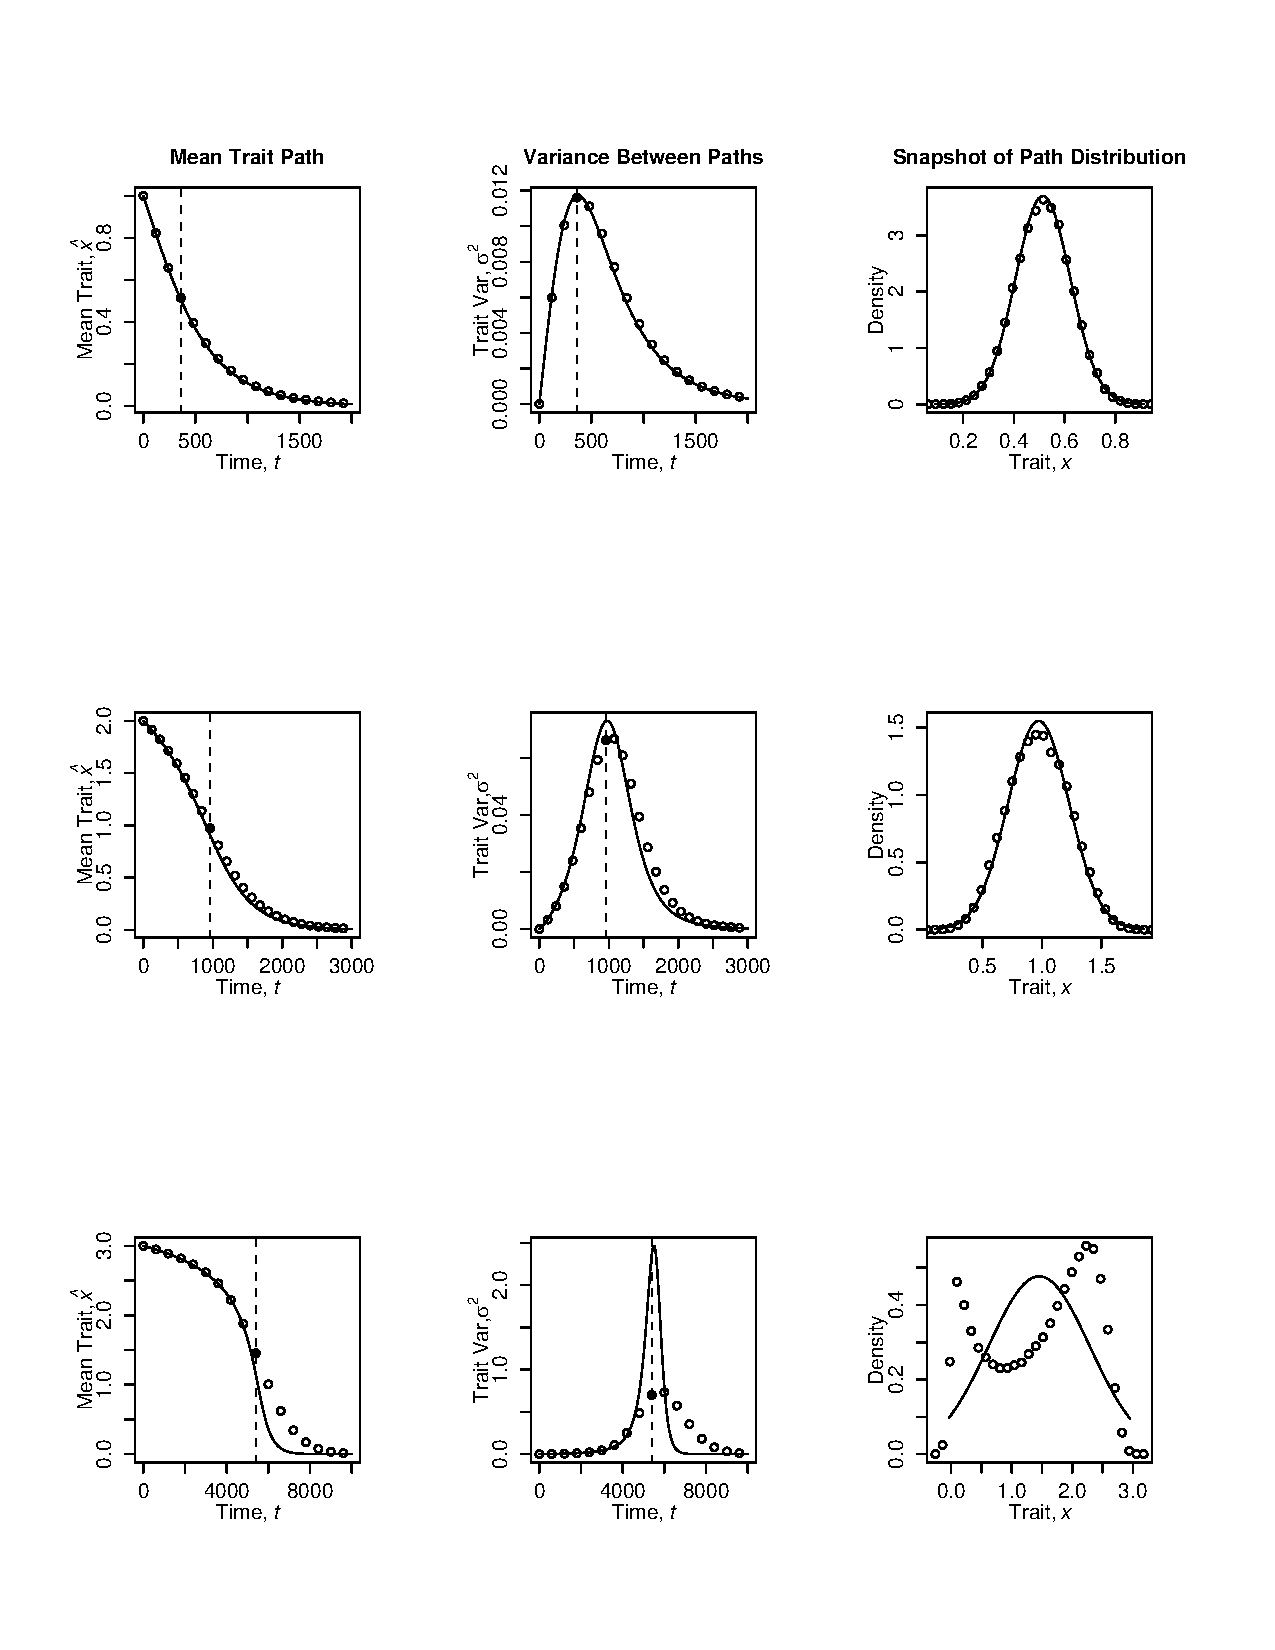
\includegraphics[width=6in]{../fallacy/figure2}
  \end{center}
  \caption{The distribution of the correlation statistic $\tau$ for two
  early warning indicators (variance, autocorrelation) on replicates
  conditionally selected for having collapsed by chance in simulations
  is shown in grey bars.  Solid lines indicate the estimated density of
  the statistic from a random sample of the simulations (not conditional
  on observing a transition). Positive values of $\tau$ correspond to
  a pattern of an indicator increasing with time; typically taken as
  evidence that a system is approaching a critical transition.  In these
  simulations, the pattern arises instead from the Prosecutor's fallacy
  of conditional selection.}
  \label{fig:indicator}
\end{figure}


For each of these replicates we also take a model-based
approach, estimating parameters for an approximate linear
model of the system approaching a saddle node bifurcation, as
described~\citet{Boettiger2012b}.  In this model, the parameter $m$
describes the approach towards the saddle-node bifurcation.  Estimates
$m < 0 $ are expected in systems approaching a bifurcation, while for
stable systems $m$ should be approximately zero. None of the estimates
across the 266 simulations differed from zero in our study, hence the
model-based estimation shows no evidence of bias on data that has been
selected conditional on collapse.



\section{Discussion}


We have shown that systems which undergo rare sudden transitions look
statistically different from their counterparts that do not, even though
they are driven by the same stochastic process.  In particular, such
conditionally selected examples are more likely to show signs associated
with an early warning of an approaching tipping point, such as increasing
variance or increasing autocorrelation, as measured by Kendall's $\tau$.
This increases the risk of false positives -- cases in which a warning
signal being tested appears to have successfully detected an oncoming
tipping point, when in fact the example comes
instead from a stable system. Figure 2 shows the extent of this bias,
where many of the chance crashes show values of $\tau$ that are 
significantly larger than those observed in the otherwise identical
replicates that did not experience a chance transition.  


\subsection{Chance transitions are false positives for early warning signals}

It seems tempting to argue that the bias towards positive detection
in historical examples is not problematic -- each of these systems did
indeed collapse, so the increased probability
of exhibiting warning signals could be taken as a successful detection.
Unfortunately this is not the case. At the moment the forecast is made,
these systems are no more likely to crash than their counterparts from
the sample that did not collapse, just as a fair coin is still a fair
coin after a string of consecutive ``heads.''  A closer look at
the patterns involved shows why common indicators
such as autocorrelation and variance can be misleading.

As the system gets farther from its stable point, it it more likely to draw a random step that
returns it towards the stable point. Despite this, there is always some probability that
it will move further still, so systems that do cross the tipping point must do
so rather quickly by a string of events.  This pattern, clearly visible before the crashes in each of
the examples in Figure 1, produces a string of observations that appear
more highly autocorrelated (if we are sampling the system frequently
enough to catch the excursion at all) than we observe in the rest of the
fluctuations around the equilibrium.  Yet this autocorrelation comes from
a chance trajectory moving quickly \emph{away} from the stable state,
not from the critical slowing down pattern in the return times to the
stable state which precede a saddle-node bifurcation and motivate the
early warning signal.


This longer than expected excursion results in a higher than expected
variance in that window as well. Both variance and autocorrelation are
calculated using a moving window over the time-series, which allows
the method to pick out a pattern of change as the window moves along
the sequence. If this chance excursion that precedes the crash happens
to fill a significant part of the moving window, the resulting pattern
will tend to show an increase in autocorrelation or variance.  If the
chance excursion is relatively rapid compared to the frequency at which
the system is observed (spacing of the data) or the width of the moving
window, the excursion may not significantly alter the general pattern.
In this way, some of the events in which a crash is observed will
appear to present these statistical patterns of increased variance
or autocorrelation without being harbingers of approaching critical
transitions.


\subsection{Comparing to the model-based method}

In our numerical experiment, the model-based estimate of early warning signals
appears more robust than the summary statistics, producing the same
estimates on both the conditionally selected replicates as on a random
sample of the replicates.  This is a consequence of the more rigid
specifications that come with a model-based approach -- the pattern
expected is less general than any increase in variance or autocorrelation,
but instead must be one that matches its approximation of the saddle-node
bifurcation. This observation highlights the difference between the
pattern driving the false positive trends in increasing variance and
increasing autocorrelation and the pattern anticipated in the saddle-node
model. This should not however be taken as evidence that the model-based
approach is immune to the bias of the Prosecutor's Fallacy.


The problem we highlight ultimately stems from the difficulty of having
only a single realization with which to examine a complex problem.
The only way to deal with this problem embodied is through replication, as
can be done in an experimental system in laboratory manipulations
such as~\citet{Drake2010, Veraart2011, Dai2012} and at the scale of whole lake
ecosystems in~\citet{Carpenter2011}.  
Experimental procedures avoid the hazard of the Prosecutor's fallacy by
generating a complete sample of replicates, rather than selecting a subset
of cases from some larger historical sample.  
%We note as well that the Prosecutors Fallacy 
%may arise in other contexts where we search historical data for
%examples containing some feature of interest.




 \section{Acknowledgements}
This research was supported by funding from NSF Grant EF 0742674 to AH
and a Computational Sciences Graduate Fellowship from the Department of
Energy grant DE-FG02-97ER25308 to CB. The authors thank M. Baskett, 
T.A. Perkins and N. Ross for helpful comments on earlier drafts of the
manuscript.  



% BOILERPLATE - Allows for individual chapters to be compiled.
%
% Usage:
%    % BOILERPLATE - Allows for individual chapters to be compiled.
%
% Usage:
%    % BOILERPLATE - Allows for individual chapters to be compiled.
%
% Usage:
%    \input{../settings/boilerplate} % place at start and end of chapter
% 

\def\precommands{%
    \input{../settings/phdsetup}
    \def\preinserted{}
    \begin{document}
}

\def\postcommands{%
    \singlespacing
    \phantomsection
%    \bibliographystyle{../bibliography/expanded}
   \bibliographystyle{elsarticle-harv}
   \bibliography{../bibliography/references}
    \enddocument
}

\def\autoinsert{%
    \ifx\preinserted\undefined
        \expandafter\precommands
    \else
        \expandafter\postcommands
    \fi
}

\ifx\master\undefined\expandafter\autoinsert\fi

 % place at start and end of chapter
% 

\def\precommands{%
    % [ USER VARIABLES ]

\def\PHDTITLE {Regime shifts in ecology and evolution}
\def\PHDAUTHOR{Carl Boettiger}
\def\PHDSCHOOL{University of California, Davis}

\def\PHDMONTH {September}
\def\PHDYEAR  {2012}
\def\PHDDEPT {Center for Population Biology}

\def\BSSCHOOL {Princeton}
\def\BSYEAR   {2007}

\def\PHDCOMMITTEEA{Alan Hastings}
\def\PHDCOMMITTEEB{Peter Wainwright}
\def\PHDCOMMITTEEC{Brian Moore}

% [ GLOBAL SETUP ]

\documentclass[letterpaper,oneside,11pt]{report}


% [ CARL BOETTIGER`S CUSTOM COMMANDS, LIBRARIES, ETC ]

\usepackage{subfigure}
\usepackage[sort&compress]{natbib}
\usepackage{color}
\usepackage{fancyvrb}
\usepackage{ctable}


\usepackage{silence}
\WarningFilter{amsmath}{Underfull}     

%\newcommand{\argmax}{\operatorname{argmax}}
\newcommand{\ud}{\mathrm{d}}


\usepackage{calc}
\usepackage{breakcites}
\usepackage[newcommands]{ragged2e}
\usepackage{appendix}
\usepackage{comment}
\usepackage{xifthen}

\usepackage{graphicx}
\usepackage{epstopdf}


\renewenvironment{abstract}{\chapter*{Abstract}}{}
\renewcommand{\bibname}{Bibliography}
\renewcommand{\contentsname}{Table of Contents}

\makeatletter
\renewcommand{\@biblabel}[1]{\textsc{#1}}
\makeatother

% [ FONT SETTINGS ]

\usepackage[T1]{fontenc}
\usepackage{libertine}

\usepackage[tbtags, intlimits, namelimits]{amsmath}
\usepackage{amsthm}
\usepackage{amssymb}
\usepackage{amsfonts}



% [ PAGE LAYOUT ]

\usepackage{geometry}
\geometry{lmargin = 1.5in}
\geometry{rmargin = 1.0in}
\geometry{tmargin = 1.0in}
\geometry{bmargin = 1.0in}

% [ PDF SETTINGS ]

\usepackage[final]{hyperref}
\hypersetup{
    breaklinks  = {true},
    colorlinks  = {true},
    linktocpage = {false},
    linkcolor   = {blue},
    citecolor   = {black},
    urlcolor    = {black},
    plainpages  = {false},
    pageanchor  = {true},
    pdfauthor   = {\PHDAUTHOR},
    pdftitle    = {\PHDTITLE},
    pdfsubject  = {Dissertation, \PHDSCHOOL},
    pdfcreator  = {},
    pdfkeywords = {},
    pdfproducer = {}
}
\urlstyle{same}

% [ LETTER SPACING ]

\usepackage[final]{microtype}
\microtypesetup{protrusion=compatibility}
\microtypesetup{expansion=false}

\newcommand{\upper}[1]{\MakeUppercase{#1}}
\let\lsscshape\scshape

\ifcase\pdfoutput\else\microtypesetup{letterspace=15}
\renewcommand{\scshape}{\lsscshape\lsstyle}
\renewcommand{\upper}[1]{\textls[50]{\MakeUppercase{#1}}}\fi

% [ LINE SPACING ]

\usepackage[doublespacing]{setspace}
\renewcommand{\displayskipstretch}{0.75}

\setlength{\parskip   }{0em}
\setlength{\parindent }{2em}

% [ TABLE FORMATTING ]

\usepackage{booktabs}
\usepackage{multirow}
\usepackage{dcolumn}
\setlength{\heavyrulewidth}{1.5\arrayrulewidth}
\setlength{\lightrulewidth}{1.0\arrayrulewidth}
\setlength{\doublerulesep }{2.0\arrayrulewidth}

% [ SECTION FORMATTING ]

\usepackage[largestsep,nobottomtitles*]{titlesec}
\renewcommand{\bottomtitlespace}{0.75in}

\titleformat{\chapter}[display]%
    {\bfseries\huge\singlespacing}%
    {\filleft\textsc{\LARGE \chaptertitlename\ \thechapter}}%
    {-0.2ex}{\titlerule[3pt]\vspace{0.2ex}}[]

\titleformat{\section}{\LARGE}{\thesection\hspace{0.5em}}{0ex}{}
\titleformat{\subsection}{\Large}{\thesubsection\hspace{0.5em}}{0ex}{}
\titleformat{\subsubsection}{\large}{\thesubsubsection\hspace{0.5em}}{0ex}{}

\titlespacing*{\chapter}{0em}{6ex}{4ex plus 2ex minus 0ex}
\titlespacing*{\section}{0em}{2ex plus 3ex minus 1ex}{0.5ex plus 0.5ex minus 0.5ex}
\titlespacing*{\subsection}{0ex}{2ex plus 3ex minus 1ex}{0ex}
\titlespacing*{\subsubsection}{0ex}{2ex plus 0ex minus 1ex}{0ex}

% [ HEADER SETTINGS ]

\usepackage{fancyhdr}

\setlength{\headheight}{\normalbaselineskip}
\setlength{\footskip  }{0.5in}
\setlength{\headsep   }{0.5in-\headheight}

\fancyheadoffset[R]{0.5in}
\renewcommand{\headrulewidth}{0pt}
\renewcommand{\footrulewidth}{0pt}

\newcommand{\pagebox}{\parbox[r][\headheight][t]{0.5in}{\hspace\fill\thepage}}

\newcommand{\prelimheaders}{\ifx\prelim\undefined\renewcommand{\thepage}{\textit{\roman{page}}}\fancypagestyle{plain}{\fancyhf{}\fancyfoot[L]{\makebox[\textwidth-0.5in]{\thepage}}}\pagestyle{plain}\def\prelim{}\fi}

\newcommand{\normalheaders}{\renewcommand{\thepage}{\arabic{page}}\fancypagestyle{plain}{\fancyhf{}\fancyhead[R]{\pagebox}}\pagestyle{plain}}

\normalheaders{}

% [ CUSTOM COMMANDS ]

\newcommand{\signaturebox}[1]{\multicolumn{1}{p{4in}}{\vspace{3ex}}\\\midrule #1\\}

% Redefine AMS proof environment to have itshape
% Note: This environment automatically adds \qed at the end. If your proof
% ends in a math environment, the \qed is placed, undesirably, on a new line.
% To prevent that, insert \qedhere inside the math environment.
\makeatletter
\renewenvironment{proof}[1][\proofname]{%
\par\pushQED{\qed}\normalfont%
\topsep6\p@\@plus6\p@\relax\trivlist%
\item[\hskip\labelsep\bfseries#1\@addpunct{.}]\itshape\ignorespaces}{%
\popQED\endtrivlist\@endpefalse}%
\makeatother

% TUGboat, Volume 0 (2001), No. 0
% http://math.arizona.edu/~aprl/publications/mathclap/perlis_mathclap_24Jun2003.pdf
% For comparison, here are the existing overlap macros:
% \def\llap#1{\hbox to 0pt{\hss#1}}
% \def\rlap#1{\hbox to 0pt{#1\hss}}
\def\clap#1{\hbox to 0pt{\hss#1\hss}}
\def\mathllap{\mathpalette\mathllapinternal}
\def\mathrlap{\mathpalette\mathrlapinternal}
\def\mathclap{\mathpalette\mathclapinternal}
\def\mathllapinternal#1#2{%
\llap{$\mathsurround=0pt#1{#2}$}}
\def\mathrlapinternal#1#2{%
\rlap{$\mathsurround=0pt#1{#2}$}}
\def\mathclapinternal#1#2{%
\clap{$\mathsurround=0pt#1{#2}$}}

\newcommand{\alert}[1]{\textbf{\textcolor{red}{#1}}}




% [ Code blocks ]
%\DefineShortVerb[commandchars=\\\{\}]{\|}
\DefineVerbatimEnvironment{Highlighting}{Verbatim}{commandchars=\\\{\}}
% Add ',fontsize=\small' for more characters per line
\newenvironment{Shaded}{}{}
\newcommand{\KeywordTok}[1]{\textcolor[rgb]{0.00,0.44,0.13}{\textbf{{#1}}}}
\newcommand{\DataTypeTok}[1]{\textcolor[rgb]{0.56,0.13,0.00}{{#1}}}
\newcommand{\DecValTok}[1]{\textcolor[rgb]{0.25,0.63,0.44}{{#1}}}
\newcommand{\BaseNTok}[1]{\textcolor[rgb]{0.25,0.63,0.44}{{#1}}}
\newcommand{\FloatTok}[1]{\textcolor[rgb]{0.25,0.63,0.44}{{#1}}}
\newcommand{\CharTok}[1]{\textcolor[rgb]{0.25,0.44,0.63}{{#1}}}
\newcommand{\StringTok}[1]{\textcolor[rgb]{0.25,0.44,0.63}{{#1}}}
\newcommand{\CommentTok}[1]{\textcolor[rgb]{0.38,0.63,0.69}{\textit{{#1}}}}
\newcommand{\OtherTok}[1]{\textcolor[rgb]{0.00,0.44,0.13}{{#1}}}
\newcommand{\AlertTok}[1]{\textcolor[rgb]{1.00,0.00,0.00}{\textbf{{#1}}}}
\newcommand{\FunctionTok}[1]{\textcolor[rgb]{0.02,0.16,0.49}{{#1}}}
\newcommand{\RegionMarkerTok}[1]{{#1}}
\newcommand{\ErrorTok}[1]{\textcolor[rgb]{1.00,0.00,0.00}{\textbf{{#1}}}}
\newcommand{\NormalTok}[1]{{#1}}



    \def\preinserted{}
    \begin{document}
}

\def\postcommands{%
    \singlespacing
    \phantomsection
%    \bibliographystyle{../bibliography/expanded}
   \bibliographystyle{elsarticle-harv}
   \bibliography{../bibliography/references}
    \enddocument
}

\def\autoinsert{%
    \ifx\preinserted\undefined
        \expandafter\precommands
    \else
        \expandafter\postcommands
    \fi
}

\ifx\master\undefined\expandafter\autoinsert\fi

 % place at start and end of chapter
% 

\def\precommands{%
    % [ USER VARIABLES ]

\def\PHDTITLE {Regime shifts in ecology and evolution}
\def\PHDAUTHOR{Carl Boettiger}
\def\PHDSCHOOL{University of California, Davis}

\def\PHDMONTH {September}
\def\PHDYEAR  {2012}
\def\PHDDEPT {Center for Population Biology}

\def\BSSCHOOL {Princeton}
\def\BSYEAR   {2007}

\def\PHDCOMMITTEEA{Alan Hastings}
\def\PHDCOMMITTEEB{Peter Wainwright}
\def\PHDCOMMITTEEC{Brian Moore}

% [ GLOBAL SETUP ]

\documentclass[letterpaper,oneside,11pt]{report}


% [ CARL BOETTIGER`S CUSTOM COMMANDS, LIBRARIES, ETC ]

\usepackage{subfigure}
\usepackage[sort&compress]{natbib}
\usepackage{color}
\usepackage{fancyvrb}
\usepackage{ctable}


\usepackage{silence}
\WarningFilter{amsmath}{Underfull}     

%\newcommand{\argmax}{\operatorname{argmax}}
\newcommand{\ud}{\mathrm{d}}


\usepackage{calc}
\usepackage{breakcites}
\usepackage[newcommands]{ragged2e}
\usepackage{appendix}
\usepackage{comment}
\usepackage{xifthen}

\usepackage{graphicx}
\usepackage{epstopdf}


\renewenvironment{abstract}{\chapter*{Abstract}}{}
\renewcommand{\bibname}{Bibliography}
\renewcommand{\contentsname}{Table of Contents}

\makeatletter
\renewcommand{\@biblabel}[1]{\textsc{#1}}
\makeatother

% [ FONT SETTINGS ]

\usepackage[T1]{fontenc}
\usepackage{libertine}

\usepackage[tbtags, intlimits, namelimits]{amsmath}
\usepackage{amsthm}
\usepackage{amssymb}
\usepackage{amsfonts}



% [ PAGE LAYOUT ]

\usepackage{geometry}
\geometry{lmargin = 1.5in}
\geometry{rmargin = 1.0in}
\geometry{tmargin = 1.0in}
\geometry{bmargin = 1.0in}

% [ PDF SETTINGS ]

\usepackage[final]{hyperref}
\hypersetup{
    breaklinks  = {true},
    colorlinks  = {true},
    linktocpage = {false},
    linkcolor   = {blue},
    citecolor   = {black},
    urlcolor    = {black},
    plainpages  = {false},
    pageanchor  = {true},
    pdfauthor   = {\PHDAUTHOR},
    pdftitle    = {\PHDTITLE},
    pdfsubject  = {Dissertation, \PHDSCHOOL},
    pdfcreator  = {},
    pdfkeywords = {},
    pdfproducer = {}
}
\urlstyle{same}

% [ LETTER SPACING ]

\usepackage[final]{microtype}
\microtypesetup{protrusion=compatibility}
\microtypesetup{expansion=false}

\newcommand{\upper}[1]{\MakeUppercase{#1}}
\let\lsscshape\scshape

\ifcase\pdfoutput\else\microtypesetup{letterspace=15}
\renewcommand{\scshape}{\lsscshape\lsstyle}
\renewcommand{\upper}[1]{\textls[50]{\MakeUppercase{#1}}}\fi

% [ LINE SPACING ]

\usepackage[doublespacing]{setspace}
\renewcommand{\displayskipstretch}{0.75}

\setlength{\parskip   }{0em}
\setlength{\parindent }{2em}

% [ TABLE FORMATTING ]

\usepackage{booktabs}
\usepackage{multirow}
\usepackage{dcolumn}
\setlength{\heavyrulewidth}{1.5\arrayrulewidth}
\setlength{\lightrulewidth}{1.0\arrayrulewidth}
\setlength{\doublerulesep }{2.0\arrayrulewidth}

% [ SECTION FORMATTING ]

\usepackage[largestsep,nobottomtitles*]{titlesec}
\renewcommand{\bottomtitlespace}{0.75in}

\titleformat{\chapter}[display]%
    {\bfseries\huge\singlespacing}%
    {\filleft\textsc{\LARGE \chaptertitlename\ \thechapter}}%
    {-0.2ex}{\titlerule[3pt]\vspace{0.2ex}}[]

\titleformat{\section}{\LARGE}{\thesection\hspace{0.5em}}{0ex}{}
\titleformat{\subsection}{\Large}{\thesubsection\hspace{0.5em}}{0ex}{}
\titleformat{\subsubsection}{\large}{\thesubsubsection\hspace{0.5em}}{0ex}{}

\titlespacing*{\chapter}{0em}{6ex}{4ex plus 2ex minus 0ex}
\titlespacing*{\section}{0em}{2ex plus 3ex minus 1ex}{0.5ex plus 0.5ex minus 0.5ex}
\titlespacing*{\subsection}{0ex}{2ex plus 3ex minus 1ex}{0ex}
\titlespacing*{\subsubsection}{0ex}{2ex plus 0ex minus 1ex}{0ex}

% [ HEADER SETTINGS ]

\usepackage{fancyhdr}

\setlength{\headheight}{\normalbaselineskip}
\setlength{\footskip  }{0.5in}
\setlength{\headsep   }{0.5in-\headheight}

\fancyheadoffset[R]{0.5in}
\renewcommand{\headrulewidth}{0pt}
\renewcommand{\footrulewidth}{0pt}

\newcommand{\pagebox}{\parbox[r][\headheight][t]{0.5in}{\hspace\fill\thepage}}

\newcommand{\prelimheaders}{\ifx\prelim\undefined\renewcommand{\thepage}{\textit{\roman{page}}}\fancypagestyle{plain}{\fancyhf{}\fancyfoot[L]{\makebox[\textwidth-0.5in]{\thepage}}}\pagestyle{plain}\def\prelim{}\fi}

\newcommand{\normalheaders}{\renewcommand{\thepage}{\arabic{page}}\fancypagestyle{plain}{\fancyhf{}\fancyhead[R]{\pagebox}}\pagestyle{plain}}

\normalheaders{}

% [ CUSTOM COMMANDS ]

\newcommand{\signaturebox}[1]{\multicolumn{1}{p{4in}}{\vspace{3ex}}\\\midrule #1\\}

% Redefine AMS proof environment to have itshape
% Note: This environment automatically adds \qed at the end. If your proof
% ends in a math environment, the \qed is placed, undesirably, on a new line.
% To prevent that, insert \qedhere inside the math environment.
\makeatletter
\renewenvironment{proof}[1][\proofname]{%
\par\pushQED{\qed}\normalfont%
\topsep6\p@\@plus6\p@\relax\trivlist%
\item[\hskip\labelsep\bfseries#1\@addpunct{.}]\itshape\ignorespaces}{%
\popQED\endtrivlist\@endpefalse}%
\makeatother

% TUGboat, Volume 0 (2001), No. 0
% http://math.arizona.edu/~aprl/publications/mathclap/perlis_mathclap_24Jun2003.pdf
% For comparison, here are the existing overlap macros:
% \def\llap#1{\hbox to 0pt{\hss#1}}
% \def\rlap#1{\hbox to 0pt{#1\hss}}
\def\clap#1{\hbox to 0pt{\hss#1\hss}}
\def\mathllap{\mathpalette\mathllapinternal}
\def\mathrlap{\mathpalette\mathrlapinternal}
\def\mathclap{\mathpalette\mathclapinternal}
\def\mathllapinternal#1#2{%
\llap{$\mathsurround=0pt#1{#2}$}}
\def\mathrlapinternal#1#2{%
\rlap{$\mathsurround=0pt#1{#2}$}}
\def\mathclapinternal#1#2{%
\clap{$\mathsurround=0pt#1{#2}$}}

\newcommand{\alert}[1]{\textbf{\textcolor{red}{#1}}}




% [ Code blocks ]
%\DefineShortVerb[commandchars=\\\{\}]{\|}
\DefineVerbatimEnvironment{Highlighting}{Verbatim}{commandchars=\\\{\}}
% Add ',fontsize=\small' for more characters per line
\newenvironment{Shaded}{}{}
\newcommand{\KeywordTok}[1]{\textcolor[rgb]{0.00,0.44,0.13}{\textbf{{#1}}}}
\newcommand{\DataTypeTok}[1]{\textcolor[rgb]{0.56,0.13,0.00}{{#1}}}
\newcommand{\DecValTok}[1]{\textcolor[rgb]{0.25,0.63,0.44}{{#1}}}
\newcommand{\BaseNTok}[1]{\textcolor[rgb]{0.25,0.63,0.44}{{#1}}}
\newcommand{\FloatTok}[1]{\textcolor[rgb]{0.25,0.63,0.44}{{#1}}}
\newcommand{\CharTok}[1]{\textcolor[rgb]{0.25,0.44,0.63}{{#1}}}
\newcommand{\StringTok}[1]{\textcolor[rgb]{0.25,0.44,0.63}{{#1}}}
\newcommand{\CommentTok}[1]{\textcolor[rgb]{0.38,0.63,0.69}{\textit{{#1}}}}
\newcommand{\OtherTok}[1]{\textcolor[rgb]{0.00,0.44,0.13}{{#1}}}
\newcommand{\AlertTok}[1]{\textcolor[rgb]{1.00,0.00,0.00}{\textbf{{#1}}}}
\newcommand{\FunctionTok}[1]{\textcolor[rgb]{0.02,0.16,0.49}{{#1}}}
\newcommand{\RegionMarkerTok}[1]{{#1}}
\newcommand{\ErrorTok}[1]{\textcolor[rgb]{1.00,0.00,0.00}{\textbf{{#1}}}}
\newcommand{\NormalTok}[1]{{#1}}



    \def\preinserted{}
    \begin{document}
}

\def\postcommands{%
    \singlespacing
    \phantomsection
%    \bibliographystyle{../bibliography/expanded}
   \bibliographystyle{elsarticle-harv}
   \bibliography{../bibliography/references}
    \enddocument
}

\def\autoinsert{%
    \ifx\preinserted\undefined
        \expandafter\precommands
    \else
        \expandafter\postcommands
    \fi
}

\ifx\master\undefined\expandafter\autoinsert\fi



